%! Author = borisdeletic
%! Date = 11/05/2023

% Preamble
\documentclass[11pt]{article}

% Document
\begin{document}

\section{Numerical Results}\label{sec:numerical_results}
    The CHMC for nested sampling algorithm was implemented as an optimised C++ library in order to run large scale,
    high dimensional tests.
    We provide a novel application of nested sampling to $\phi^4$-theory to perform experiments.
    The $\phi^4$ action was given as the likelihood function as defined in section~\ref{subsec:nested-sampling-phi4}.

    All input parameter values are listed in appendix~\ref{sec:param_table} and full details about the implementation
    can be found in appendix~\ref{sec:code_implementation}.
    All results were gathered using a single core on the CSD3 compute cluster.

\subsection{Phase Transitions}\label{subsec:phase_transition}
    To investigate the phase transition in $\phi^4$-theory, we aim to measure the mean magnetisation~\eqref{eq:magnetization}
    of the field for a wide range of $\kappa$ \& $\lambda$ values.

    We use a $32 \times 32$ lattice ($D=1024$) and set $n_{\text{live}}=500$ with precision criteria $p=0.1$.
    For this setup, the average number of nested sampling iterations to converge is $i_{\max} \approx 15,000$.

    We vary the action~\eqref{eq:phi4_action} across the range $\kappa \in (0, 0.3), \quad \lambda \in (0, 0.03)$ for
    a total of $1,000$ unique actions, and calculate $\langle M \rangle$ for each one to construct a phase diagram.

    \begin{figure}[h!]
        \center
        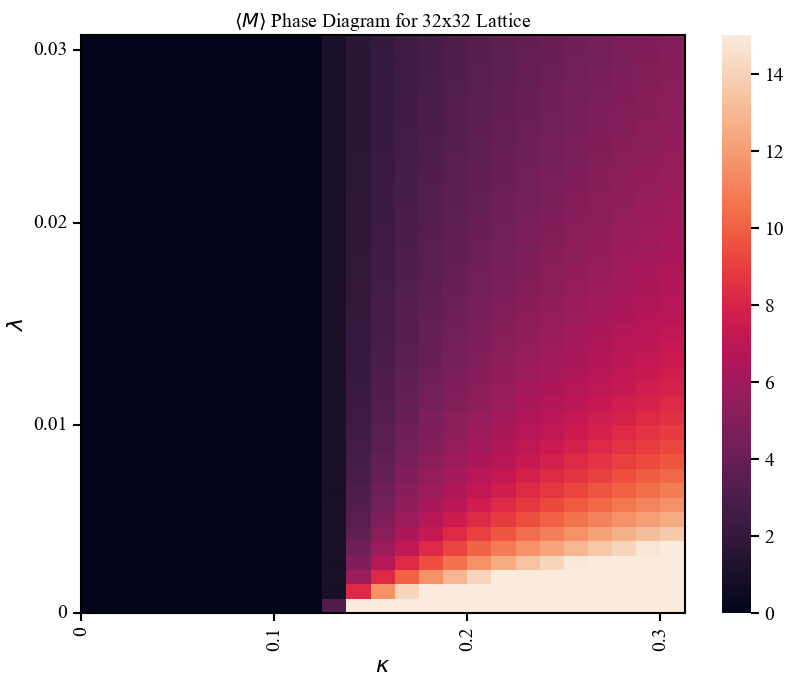
\includegraphics[width=\linewidth]{../figures/PhaseDiagram}
        \caption{
            $\kappa$ vs $\lambda$ phase diagram for 32x32 lattice $\phi^4$-theory.
            For $\kappa \lesssim 0.125$, we see the expression of the disordered phase with $\langle M \rangle = 0$.
            The second-order phase transition is apparent along this boundary, as $\langle M \rangle$ grows suddenly
            across it. \\
            In the ordered phase ($\kappa \gtrsim 0.125$), the mean magnetisation is strongly dependent on the field
            coupling $\lambda$.
            With a weak coupling, the kinetic energy dominates and the field seperates, leading to
            large $\langle M \rangle$.
            We also note that $\lambda$ has a minor influence on the exact critical point in $\kappa$, with the
            critical line having a slight negative slope.
        }\label{fig:phase_diagram}
    \end{figure}

    This phase diagram accurately reconstructs the theoretical result and is verified against other
    simulations~\cite{Pawlowski_2020}.

\subsection{Correlation Functions}\label{subsec:correlation_function}
    The two-point correlation functions are a key quantity related to physical
    observables of the quantum field theory.
    For example, the renormalised mass parameter and correlation length can both be measured with correlation
    functions~\cite{maas2020lattice,brower2018lattice}.

    In the context of a Euclidean $\phi^4$ theory, we define the spatial (equal-time) correlation functions as
    \begin{equation}\label{eq:full_correlation_function}
    C(x_1, x_2) = \langle \phi(x_1) \phi(x_2) \rangle,
    \end{equation}
    where $\langle . \rangle$ denotes the Markov-Chain ensemble average~\eqref{eq:mcmc_observable}.

    Exploiting the translational and rotational symmetry of the $\phi^4$ action, we can fully characterise the two-point
    correlation function in terms of the distance between two points $r$
    \begin{equation}\label{eq:correlation_function}
    C(r) = \langle \phi(x) \phi(x + r) \rangle,
    \end{equation}
    where we now also average over all lattice points $x$.

    Directly calculating correlation functions numerically is prohibitively expensive, requiring $\mathcal{O}(N^3)$
    operations for each microstate.
    Therefore, we use a method of fourier transform and convolution theorem to speed up
    calculation~\cite{Ruge_1994}.

    In the continuous limit $N \rightarrow \infty$ we can write the correlation function for a single microstate at
    Markov-Chain iteration $i$ as
    \begin{equation}\label{eq:continuous_correlation}
        C_{i}(r) = \int_{-\infty}^{\infty} \phi(x) \phi(x + r) dx.
    \end{equation}

    Applying the convolution theorem gives
    \begin{equation}\label{eq:convolution_theorem}
        C_{i}(r) = \mathcal{F}^{-1} \{ |\tilde{\phi}(k)|^2 \}
    \end{equation}
    providing a new way to evaluate the correlation function.
    Using a discrete fast fourier transform, we can therefore calculate the correlation function in
    $\mathcal{O}(N^2 \log N)$.

    Just below the critical point, the correlation function decays exponentially as $C(r) \sim \exp(-r / \xi)$,
    where $\xi$ is defined as the correlation length.
    At the critical point, the correlation length diverges and becomes infinite in the ordered phase.

    We measure the correlation functions on a large 512x512 lattice ($D=262,144$) to minimise finite-size effects which
    will cause significant errors for smaller lattices.
    Using $n_{\text{live}}=200$ sped up the computation time to average $5,000$ iterations per lattice and still
    provided high resolution results.

    With fixed $\lambda=0.03$, we show the measured correlation functions for a range
    of $\kappa$ up to the critical point.

\begin{figure}[h!]
    \center
    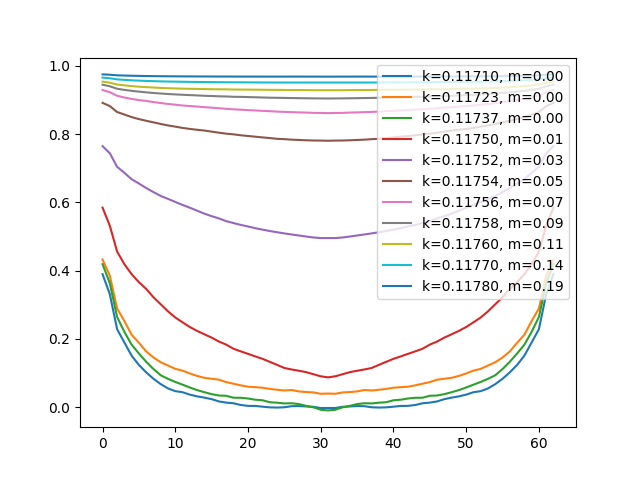
\includegraphics[width=\linewidth]{../figures/correlations_n64}
    \caption{
        64x64 lattice correlation functions.
    }\label{fig:correlation_functions}
\end{figure}


\subsection{Critical Slowing Down}\label{subsec:critical_slowing_down}
We observe that the number of iterations required to converge is not dramatically higher as we approach criticality.
The algorithm successfully samples and estimates observables accurately at the critical point, without any
modifications or difficulty.
This confirms the expected behaviour that leveraging nested sampling provides strong resistance to topological freezing.

\end{document}
